%%%%%%%%%%%%%%%%%%%%%%%%%%%%%%%%%%%%%%%%%%%%%%%%%%%%%%%%%%%%%%%%%%%%%%%%%%%%%%%
\documentclass[hyperref={pdfpagelabels=false},compress,table]{beamer} % 在Mac下无法编译
% \documentclass[compress,table]{beamer} % 在Mac下使用
% package for font
\usepackage{fontspec}
\defaultfontfeatures{Mapping=tex-text}  %%如果没有它,会有一些 tex 特殊字符无法正常使用,比如连字符。
\usepackage{xunicode,xltxtra}
\usepackage[BoldFont,SlantFont,CJKnumber,CJKchecksingle]{xeCJK}  % \CJKnumber{12345}: 一万二千三百四十五
\usepackage{CJKfntef}  %%实现对汉字加点、下划线等。
\usepackage{pifont}  % \ding{}
% package for math
\usepackage{amsfonts}

% package for graphics
\usepackage[americaninductors,europeanresistors]{circuitikz}
\usepackage{tikz}
\usetikzlibrary{plotmarks}  % placements=positioning
\usepackage{graphicx}  % \includegraphics[]{}
\usepackage{subfigure}  %%图形或表格并排排列
% package for table
\usepackage{colortbl,dcolumn}  %% 彩色表格
\usepackage{multirow}
\usepackage{multicol}
\usepackage{booktabs}
% package for code
\usepackage{fancyvrb}
\usepackage{listings}

% \usepackage{animate}
% \usepackage{movie15}

%%%%%
% setting for beamer
\usetheme{default} % Madrid(常用), Copenhagen, AnnArbor, boxes(白色), Frankfurt,Berkeley
\useoutertheme[subsection=true]{miniframes} % 使用Berkeley时注释本行
\usecolortheme{sidebartab}
\usefonttheme{serif}  %%英文使用衬线字体
% \setbeamertemplate{background canvas}[vertical
% shading][bottom=white,top=structure.fg!7] %%背景色,上25%的蓝,过渡到下白。
\setbeamertemplate{theorems}[numbered]
\setbeamertemplate{navigation symbols}{}  %% 去掉页面下方默认的导航条
\setbeamercovered{transparent}  %设置 beamer 覆盖效果

% 设置标题title背景色
% \setbeamercolor{title}{fg=black, bg=lightgray!60!white}
\setbeamercolor{title}{fg=white, bg=black!70!white}

% 设置每页小LOGO
\pgfdeclareimage[width=1cm]{ouc}{figures/static/ouc.pdf}
\logo{\pgfuseimage{ouc}{\vspace{-20pt}}}

% setting for font
%%\setCJKmainfont{Adobe Kaiti Std}
\setCJKmainfont{SimSun} 
%% \setCJKmainfont{FangSong_GB2312} 
%% \setmainfont{Apple Garamond}  %%苹果字体没有SmallCaps
\setCJKmainfont{SimSun} 
%FUNNY%\setCJKmainfont{DFPShaoNvW5-GB}  %%华康少女文字W5(P)
%FUNNY%\setCJKmainfont{FZJingLeiS-R-GB}  %%方正静蕾体
%FUNNY%\setmainfont{Purisa}
%\setsansfont[Mapping=tex-text]{Adobe Song Std}
     %如果装了Adobe Acrobat,可在font.conf中配置Adobe字体的路径以使用其中文字体。
     %也可直接使用系统中的中文字体如SimSun、SimHei、微软雅黑等。
     %原来beamer用的字体是sans family;注意Mapping的大小写,不能写错。
     %设置字体时也可以直接用字体名,以下三种方式等同:
     %\setromanfont[BoldFont={黑体}]{宋体}
     %\setromanfont[BoldFont={SimHei}]{SimSun}
     %\setromanfont[BoldFont={"[simhei.ttf]"}]{"[simsun.ttc]"}
% setting for graphics
\graphicspath{{figures/}}  %%图片路径
\renewcommand\figurename{图}

% setting for pdf
\hypersetup{% pdfpagemode=FullScreen,%
            pdfauthor={Xiaodong Wang},%
            pdftitle={Title},%
            CJKbookmarks=true,%
            bookmarksnumbered=true,%
            bookmarksopen=false,%
            plainpages=false,%
            colorlinks=true,%
            citecolor=green,%
            filecolor=magenta,%
            linkcolor=blue,%red(default)
            urlcolor=cyan}

% setting for fontspec
\XeTeXlinebreaklocale "zh"  %%表示用中文的断行
\XeTeXlinebreakskip = 0pt plus 1pt minus 0.1pt  %%多一点调整的空间
%%%%%

% font setting by xeCJK
\setCJKfamilyfont{NSimSun}{NSimSun}
\newcommand{\song}{\CJKfamily{NSimSun}}
%%%\setCJKfamilyfont{AdobeSongStd}{Adobe Song Std}
%%%\newcommand{\AdobeSong}{\CJKfamily{AdobeSongStd}}
\setCJKfamilyfont{FangSong}{FangSong_GB2312}
\newcommand{\fang}{\CJKfamily{FangSong}}
%%%\setCJKfamilyfont{AdobeFangsongStd}{Adobe Fangsong Std}
%%%\newcommand{\AdobeFang}{\CJKfamily{AdobeFangsongStd}}
\setCJKfamilyfont{SimHei}{SimHei}
\newcommand{\hei}{\CJKfamily{SimHei}}
%%%\setCJKfamilyfont{AdobeHeitiStd}{Adobe Heiti Std}
%%%\newcommand{\AdobeHei}{\CJKfamily{AdobeHeitiStd}}
\setCJKfamilyfont{KaiTi}{KaiTi}
\newcommand{\kai}{\CJKfamily{KaiTi}}
%%%\setCJKfamilyfont{AdobeKaitiStd}{Adobe Kaiti Std}
\newcommand{\AdobeKai}{\CJKfamily{AdobeKaitiStd}}
\setCJKfamilyfont{LiSu}{LiSu}
\newcommand{\li}{\CJKfamily{LiSu}}
\setCJKfamilyfont{YouYuan}{YouYuan}
\newcommand{\you}{\CJKfamily{YouYuan}}
\setCJKfamilyfont{FZJingLei}{FZJingLeiS-R-GB}
\newcommand{\jinglei}{\CJKfamily{FZJingLei}}
\setCJKfamilyfont{MSYH}{Microsoft YaHei}
\newcommand{\msyh}{\CJKfamily{MSYH}}

% 自定义颜色
\def\Red{\color{red}}
\def\Green{\color{green}}
\def\Blue{\color{blue}}
\def\Mage{\color{magenta}}
\def\Cyan{\color{cyan}}
\def\Brown{\color{brown}}
\def\White{\color{white}}
\def\Black{\color{black}}

\lstnewenvironment{xmlCode}[1][]{% for Java
  \lstset{
    basicstyle=\tiny\ttfamily,%
    columns=flexible,%
    framexleftmargin=.7mm, %
    % frame=shadowbox,%
    % rulesepcolor=\color{cyan},%
     frame=single,%
    backgroundcolor=\color{white},%
    xleftmargin=4\fboxsep,%
    xrightmargin=4\fboxsep,%
    numbers=left,numberstyle=\tiny,%
    numberblanklines=false,numbersep=7pt,%
    language=xml, %
    }\lstset{#1}}{}

\lstnewenvironment{javaCode}[1][]{% for Java
  \lstset{
    basicstyle=\tiny\ttfamily,%
    columns=flexible,%
    framexleftmargin=.7mm, %
    frame=shadowbox,%
    rulesepcolor=\color{cyan},%
    % frame=single,%
    backgroundcolor=\color{white},%
    xleftmargin=4\fboxsep,%
    xrightmargin=4\fboxsep,%
    numbers=left,numberstyle=\tiny,%
    numberblanklines=false,numbersep=7pt,%
    language=Java, %
    }\lstset{#1}}{}

\lstnewenvironment{shCode}[1][]{% for Java
  \lstset{
    basicstyle=\scriptsize\ttfamily,%
    columns=flexible,%
    framexleftmargin=.7mm, %
    frame=shadowbox,%
    rulesepcolor=\color{brown},%
    % frame=single,%
    backgroundcolor=\color{white},%
    xleftmargin=4\fboxsep,%
    xrightmargin=4\fboxsep,%
    numbers=left,numberstyle=\tiny,%
    numberblanklines=false,numbersep=7pt,%
    language=sh, %
    }\lstset{#1}}{}

\newcommand\ask[1]{\vskip 4bp \tikz \node[rectangle,rounded corners,minimum size=6mm,
  fill=white,]{\Cyan \includegraphics[height=1.5cm]{question} \Large \msyh #1};}

\newcommand\wxd[1]{\vskip 4bp \tikz \node[rectangle,minimum size=6mm,
  fill=blue!60!white,]{\White \ding{118} \msyh #1};}

\newcommand\xyy[1]{\vskip 2bp \tikz \node[rectangle,minimum size=3mm,
  fill=black!80!white,]{\White \msyh\scriptsize #1};}

\newcommand\cxf[1]{\vskip 4bp \tikz \node[rectangle,rounded corners,minimum size=6mm,
  fill=orange!60!white,]{\White \ding{42} \msyh #1};}

\newcommand\samp[1]{\vskip 2bp \tikz \node[rectangle,minimum size=3mm,
  fill=white!100!white,]{\Mage\msyh \small CODE \ding{231} \Black #1};\vskip -8bp}

\newcommand\zhyfly[1]{\tikz \node[rectangle,rounded corners,minimum size=6mm,ball color=red!25!blue,text=white,]{#1};}

\setbeamerfont{frametitle}{series=\msyh} % 修改Beamer标题字体

\makeatletter
\newcommand{\Extend}[5]{\ext@arrow 0099{\arrowfill@#1#2#3}{#4}{#5}}
\makeatother


%%%%%%%%%%%%%%%%%%%%%%%%%%%%%%%%%%%%%%%%%%%%%%%%%%%%%%%%%%%%%%%%%%%%%%%%%%%%%%%
% \titlepage
\title[KevinW@OUC]{\hei {\huge Java EE企业应用系统开发}\\  
HTTP响应处理编程}
\author[王晓东]{王晓东\\
  \href{mailto:wangxiaodong@ouc.edu.cn}{\footnotesize wangxiaodong@ouc.edu.cn}}
\institute[中国海洋大学]{\small 中国海洋大学}
\date{\today}
\titlegraphic{\vspace{-6em}
\includegraphics[height=6cm]{static/ouc.pdf}\vspace{-6em}}
%%%%%
\begin{document}
%% Delete this, if you do not want the table of contents to pop up at
%% the beginning of each subsection:
\AtBeginSection[]{                              % 在每个Section前都会加入的Frame
  \frame<handout:0>{
    \frametitle{\textbf{\hei 接下来…}}
    \tableofcontents[currentsection]
  }
}  %

\AtBeginSubsection[]                            % 在每个子段落之前
{
  \frame<handout:0>                             % handout:0 表示只在手稿中出现
  {
    \frametitle{\textit{\hei 接下来…}}\small
    \tableofcontents[current,currentsubsection] % 显示在目录中加亮的当前章节
  }
}
 \frame{\titlepage}

%%%%%%%%%%%%%%%%%%%%%%%%%%%%%%%%%%%%%%%%%%%%%%%%
\begin{frame}
\frametitle{参考书目}
\begin{enumerate}
\item 吕海东,张坤 编著,Java EE企业级应用开发实例教程,清华大学出版社,2010年8月
\end{enumerate}  
\end{frame}

% \begin{frame}
% \frametitle{本章学习目标}
% \begin{enumerate}
% \item 
% \end{enumerate}  
% \end{frame}

\section*{大纲}
\frame{\frametitle{大纲} \tableofcontents}

\section{HTTP响应的内容}

\begin{frame}[fragile] % [fragile]参数使得能够插入代码
\frametitle{HTTP响应的内容}

在Web服务器接收请求处理后,向客户端发送HTTP响应(Response)。响应的内容包括:
\begin{itemize}
\item 响应状态(Status Code)
\item 响应头(Response Header)
\item 响应体(Response Body)
\end{itemize}

Java Web中响应由响应对象Response完成。
\end{frame}

\begin{frame}[fragile,fragile] % [fragile]参数使得能够插入代码
\frametitle{HTTP响应状态行} 

表明响应的状态信息,如成功、失败、错误。

状态行组成:版本 / 状态代码 / 状态消息。

状态行例子:
\begin{verbatim}
HTTP/1.1 200 ok
\end{verbatim}
\begin{enumerate}
\item 版本:使用的HTTP协议版本,如HTTP/1.1;
\item 状态代码:3位数字;
  \begin{itemize}
  \item 1xx: 收到请求,没有处理完。
  \item 2xx: 成功,响应完毕。
  \item 3xx:重定向,到另一个请求中去。
  \item 4xx:失败,没有请求的文档等。
  \item 5xx:内部错误,代码出现异常。
  \end{itemize}
\item 状态描述。
\end{enumerate}
\end{frame}

\begin{frame}[fragile] % [fragile]参数使得能够插入代码
\frametitle{响应头} 

Web服务器在向客户端发送HTTP响应时也可以包含响应头,赖指示客户端如何处理响应体,主要用来告诉浏览器响应的类型、字符编码和字节大小等信息,以使得浏览器知道如何处理响应内容。

常见响应头内容:
\begin{enumerate}
\item 指示HTTP响应可以接收到的文档类型集:Accept
\item 告知客户可以接收的字符集:Accept-Charset
\item 所有响应的字符编码集:Accept-Encoding
\item 响应体的MIME类型:Content-Type
\item 响应体的语言类型:Context-Language
\item 响应体的长度和字节数:Content-Length
\item 通知客户端到期时间:Expires 
\item 缓存情况:Cache-Control
\item 重定向到另一个URL地址:Redirect
\end{enumerate}
\end{frame}

\begin{frame}[fragile] % [fragile]参数使得能够插入代码
\frametitle{响应体} 

响应体类型由响应头确定,可以使任何类型。浏览器在处理响应体之前,会收到响应头,根据响应头的信息,确定如何处理响应体,如响应头的Content-Type为PDF,则浏览器会启动PDF Reader来处理此响应体以显示PDF文档。

常用类型包括:
\begin{enumerate}
\item 纯文本:text/plain
\item HTML:text/html
\item 图片:image/gif, image/jpeg
\item PDF:application/pdf
\end{enumerate}

注意:
\begin{itemize}\kai
\item 文本类型响应要求响应头中包含MIME类型和字符编码集,使用{\hei 字符输出流}向客户端发送响应体数据;
\item 二进制数据类型响应需要在响应头中包含MIME类型,不要设置字符编码集,使用{\hei 字节输出流}向客户端发送响应体数据。
\end{itemize}
\end{frame}

\section{HTTP响应对象}

\begin{frame}[fragile] % [fragile]参数使得能够插入代码
\frametitle{响应对象类型} 

\wxd{响应对象类型}

javax.servlet.http.HttpServeletResponse

\wxd{响应对象职责}

\begin{itemize}
\item 设置状态行;
\item 发送响应头 ;
\item 向Web浏览器发送HTTP响应体;
\item 控制页面的重定向,即将告知浏览器再发送一次请求。
\end{itemize}
\end{frame}

\begin{frame}[fragile] % [fragile]参数使得能够插入代码
\frametitle{响应对象生命周期} 

\begin{enumerate}
\item Web容器自动为每次Web组件的请求生成一个响应对象。
\item Web容器创建响应对象后,传入到doGet或doPost方法。
\item 通过响应对象向浏览器发响应。
\item 响应结束后,Web容器销毁响应对象,释放所占用的内存。
\end{enumerate}

\end{frame}

\section{响应对象功能和方法}

\begin{frame}[fragile] % [fragile]参数使得能够插入代码
\frametitle{设置响应状态码} 

一般情况下,Web开发人员不需要通过编程来改变响应状态码,Web服务器会根据请求处理的情况自动设置状态码,并发送到客户端浏览器。例如,当客户请求不存在的URL地址时,Web服务器会自动设置状态码为404,状态消息为not found。

\wxd{public void setStatus(int code)}

直接发送指定的响应状态码,没有设置状态消息,只有默认的状态消息,如果无对应状态消息则显示为空。

\wxd{public void setStatus(int code, String message)}

设置指定的状态码,同时设定自定义的状态消息,可以修改默认的状态消息。该方法在Servlet 2.5后被舍弃,一般不要使用。

\end{frame}

\begin{frame}[fragile] % [fragile]参数使得能够插入代码
\frametitle{设置响应状态码} 

\wxd{public void sendError(int sc) throws IOException}

向客户端发送指定的错误信息码,可以是任意定义的整数。

\begin{javaCode}
response.setCharacterEncoding("GBK");
response.sendError(580); 
\end{javaCode}

\wxd{public void sendError(int sc, String msg) throws IOException}

向客户端发送指定的错误信息码和自定义状态消息。

\begin{javaCode}
response.setCharacterEncoding("GBK");
response.sendError(580, "自定义错误"); 
\end{javaCode}
\end{frame}

\begin{frame}[fragile] % [fragile]参数使得能够插入代码
\frametitle{设置响应头} 

{\hei 当客户端接收到响应状态为200时,浏览器会继续接收响应头信息,来确定响应体的类型和大小。}

\wxd{public void setHeader(String name, String value)}

将指定名称和值的响应头发送到客户端。
\begin{javaCode}
response.setHeader("Content-Type", "text/html");  
\end{javaCode}

\wxd{public void setIntHeader(String name, int value)}

设置整数类型的响应头的名和值。 
\begin{javaCode}
response.setHeader("Content-Length", 20);  
\end{javaCode}
{\kai 实际项目中无需设定该响应头,Web服务器会自动计算并发送给浏览器。}

\wxd{public void setDateHeader(String name,long date)}

设定日期类型的响应头,参数date为GMT格式的日期。
\end{frame}

\begin{frame}[fragile] % [fragile]参数使得能够插入代码
\frametitle{设置响应头的便捷方法} 

\wxd{public void setContentType(String type)}

直接设置响应内容类型MIME响应头。

\wxd{public void setContentLength(int len)}

设置响应体长度,以字节为单位。

\wxd{void setCharacterEncoding(String charset)}

设置响应字符集,包括响应状态,响应头和响应体。 
\end{frame}

\begin{frame}[fragile] % [fragile]参数使得能够插入代码
\frametitle{设置响应头的便捷方法} 

\wxd{public void setBufferSize(int size)}

设定响应体的缓存字节数。

如设定响应体缓存为4k:
\begin{javaCode}
response.setBufferSize(4096);  
\end{javaCode}

{\kai Servlet在发送响应时,一般按照发送状态码、响应头和响应体的顺序进行,大的响应体缓存,可以允许Servlet有更多的时间发送状态码和响应头,这种情况发生在响应头和响应体同时写的情况。}

提示:编程的时候最好先把响应头全部设定后,再发送响应体。
\end{frame}

\begin{frame}[fragile] % [fragile]参数使得能够插入代码
\frametitle{响应对象方法——向客户端传送Cookie} 

\wxd{public void addCookie(Cookie cookie);}

此方法功能将Cookie对象放置在响应头中,随响应内容到浏览器客户端,并保存到客户端的PC的本地目录中。

\begin{javaCode}
Cookie cookie01=new Cookie("userid", "9001");
response.addCookie(cookie01);
\end{javaCode}

\end{frame}

\begin{frame}[fragile] % [fragile]参数使得能够插入代码
\frametitle{响应对象方法——请求重定向} 

\wxd{public void sendRedirect(String url)}

将对客户的响应重定向到新的URL上,让客户端浏览器对此URL进行请求。

{\kai 重定向到登录页面,相当于在浏览器地址栏上再输入一次URL地址,进行一次HTTP请求:}

\begin{javaCode}
 String url="../admin/login.jsp";
 response.sendRedirect(url);
 \end{javaCode}
\end{frame}

\begin{frame}[fragile] % [fragile]参数使得能够插入代码
\frametitle{设置响应体发送功能}

响应体即浏览器实际显示的具体内容,可以时HTML网页,也可以是其他文件格式,由响应头的Content-Type决定。

响应体的类型主要分为两大类,即文本类型和二进制类型。{\Red 文本类型使用字符输出流PrintWriter的对象来实现;二进制类型由OutputStream的对象来实现。}

\wxd{public PrintWriter getWriter()}

取得字符输出流。

\wxd{public ServletOutputStream getOutputStream()}

取得二进制输出流。

\end{frame}

\begin{frame}[fragile] % [fragile]参数使得能够插入代码
\frametitle{设置响应体——文本类型响应体发送编程}
\begin{enumerate}
\item 设置响应类型ContentType
\begin{javaCode}
response.setContentType("text/html"); //响应类型为 HTML 文档    
\end{javaCode}
\item 设置响应字符编码
\begin{javaCode}
response.setCharacterEncoding("GBK"); //字符编码使用 GBK
\end{javaCode}
\item 取得字符输出流对象
\begin{javaCode}
PrintWriter out = response.getWriter();
\end{javaCode}
\item 向流对象中发送文本数据
\begin{javaCode}
out.println("<html><body></body></html>"); //输出文本字符
\end{javaCode}
\item 清空流中缓存的字符
\begin{javaCode}
out.flush();
\end{javaCode}
\item 关闭流
\begin{javaCode}
out.close();
\end{javaCode}
\end{enumerate}
\end{frame}

\begin{frame}[fragile] % [fragile]参数使得能够插入代码
\frametitle{设置响应体——文本类型响应体发送编程}

\samp{示例}

\begin{javaCode}
response.setContentType("text/html; charset=gb2312");
PrintWriter out = response.getWriter();

out.println("<html><head>");
out.println("</head><body>");
out.println("hello! ");
out.println("</body></html>");
out.flush();
out.close();
\end{javaCode} 

\end{frame}

\begin{frame}[fragile] % [fragile]参数使得能够插入代码
\frametitle{设置响应体——二进制类型响应体发送编程}
\begin{enumerate}
\item 设置响应类型ContentType
\begin{javaCode}
response.setContentType("image/jpeg"); //响应类型为 JPEG 图片
\end{javaCode}

\item 取得字节输出流对象
\begin{javaCode}
OutputStream out = response.getOutputStream(); //取得字节输出流
\end{javaCode}

\item 向流对象中发送字节数据
\begin{javaCode}
out.println(200); //输出字节数据
\end{javaCode}

\item 清空流中缓存的字节
\begin{javaCode}
out.flush();
\end{javaCode}

\item 关闭流
\begin{javaCode}
out.close();
\end{javaCode}

{\Red\kai 注意:二进制响应编程不需要设置字符编码。}
\end{enumerate}
\end{frame}
%%%%%%%%%%%%%%%%%%%%%%%%%%
\begin{frame}[fragile] % [fragile]参数使得能够插入代码
\frametitle{} 

\end{frame}
%%%%%%%%%%%%%%%%%%%%%%%%%%
%% \begin{figure}
%% \centering
%% 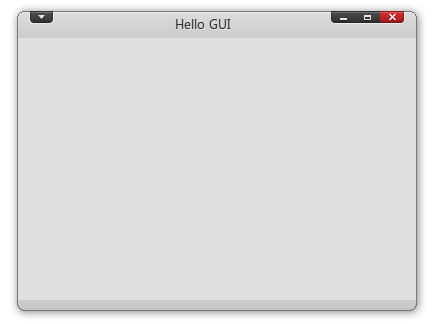
\includegraphics[width=0.6\textwidth]{fig01.png}
%% \end{figure}
% TKS %%%%%%%%%%%%%%%%%%%%%%%%%%%%%%%%%%%%%%%%%%%%%%
\begin{frame}
\centering
{\Huge \textcolor{blue}{THE END}} \\
\vspace{5mm}
{\Large wangxiaodong@ouc.edu.cn} \\
\end{frame}
%%%%%%%%%%%%%%%%%%%%%%%%%%%%%%%%%%%%%%%%%%%%%%%%%%
\end{document}
